\documentclass[12pt]{article}

\usepackage{sbc-template}

\usepackage[brazil]{babel}
\usepackage[utf8]{inputenc}

\usepackage[alf]{abntex2cite}
\usepackage{graphicx}
\usepackage{float}

\graphicspath{{\main/imagens/}{imagens/}}

\AtBeginEnvironment{quote}{\smaller} % Step font down one size relative to current font.

\sloppy

\title{\normalfont{Desenvolvimento de Documentação e Implementação de Sistema de Informação
para Auxílio na Aprendizagem de Qualidade de Software}}

\author{Vinícius B. Bruscagini\inst{1}, Carlos R. S. Júnior\inst{1}}

\address{Instituto Federal de Educação, Ciência e Tecnologia do Estado de São Paulo\\Campus Hortolândia (IFSP-HTO)
\email{vinicius.bruscagini@aluno.ifsp.edu.br, carlos.rsantos@ifsp.edu.br}}

\begin{document}

\maketitle

\begin{abstract}
  This paper has the objective to create an App using famous technologies and tools
  avaliable on the market. Applying software quality and project management concepts.
  A documentation covering all the aspects of the system will be released to help students
  and developers understand these concepts in a practical way.
\end{abstract}

\begin{resumo}
  Este trabalho possui o objetivo de criar um sistema de informação utilizando tecnologias e ferramentas
  famosas no mercado, aplicando conceitos de qualidade de software e gerenciamento de projetos.
  Será disponibilizado um material que documentará todos os aspectos desse sistema, de forma a ajudar
  estudantes e desenvolvidores a entenderem como funcionam conceitos de qualidade de software na prática.
\end{resumo}

\section{Introdução}

A área de TI, incluindo desenvolvimento de software, é uma área que evoluiu muito nas ultimas
décadas~\cite{Pacheco10} e continua evoluindo rapidamente até hoje. Novas Tecnologias e ferramentas
surgem em rítmo acelerado e muitas delas ganham popularidade, demandando assim, novas
habilidades para os profissionais de TI\@. Com essa evolução, os cursos oferecidos nessa área não conseguem
oferecer disciplinas sobre tecnologias usadas no mercado. O ensino, então, não propicia o aprendizado
suficiente para os profissionais de TI, fazendo com que muitos desses busquem cursos ou certificações para
aprimorar seus conhecimentos.~\cite{macedo09}. Além disso, de acordo com uma pesquisa realizada por
~\cite{wei08} os alunos de cursos de Engenharia de Software se preocupam em possuir um aprendizado
voltado para prática e sempre ter convivência com conceitos e métodos importantes para o mercado de trabalho.

Baseando-se nessas questões, a produção desse trabalho tem a proposta de desenvolver
um sistema com tecnologias e ferramentas populares que possuem demanda por profissionais,
com o objetivo principal de construir uma documentação
que abrange todos os aspectos desse sistema e que explique com clareza como o software
funciona, quais tecnologias foram usadas e como se deu o seu desenvolvimento.
O código fonte da aplicação e a documentação serão publicados e então esses materiais
poderiam ser consultados por qualquer pessoa, assim ajudando elas a
entenderem alguns conceitos de Desenvolvimento de Software e como se dão suas aplicações na prática.

\section{Fundamentação Teórica}

Para atingirmos um software conforme descrito na seção anterior, precisamos entender
alguns conceitos importantes dessa área.

\subsection{Framework}

Um conceito importante no desenvolvimento de sistemas é o `Framework', de acordo com~\cite{host12} um
framework é como um template que conta com diversas funcionalidades. Ele possui o objetivo principal de
resolver problemas recorrentes no desenvolvimento e acelerar esse processo. O
Projeto Pedagógico do Curso de Análise e Desenvolvimento de Sistemas do IFSP - Campus Hortolândia
contém uma disciplina que ensina o uso de um framework para o desenvolvimento. No entanto, a bibliografia básica
que aborda esse framework é do ano de 2010 e faz uso da tecnologia JSF, que hoje em dia é muito pouco usada.~\cite{webtechsurveyJSF}

% explicar o que é qualidade e arquitetura de "sistema de produção"
\subsection{Qualidade de Software}

A definição de qualidade no contexto da computação nem sempre é um consenso,
existem diferentes terminologias, as quais podem causar problemas para pessoas que não
possuem conhecimento sobre.~\cite{Duarte03}

Um software pode ser considerado de qualidade quando ele atende a todas as necessidades, explicitas
e implícitas para qual ele foi feito.~\cite{Duarte03}

Enquanto ao código, que será o foco do artigo, existem padrões que devem ser seguidos para um código
possuir qualidade. Para isso devemos pontuar que para um código ter qualidade ele deve funcionar, e principalmente,
ser légivel.

\begin{quote}
  ``Muitos programadores iniciantes acham que um bom código é aquele que é correto, ou seja, faz o que tem
  que fazer.''~\cite{Levy04}.
\end{quote}

Um código, para funcionar deve possuir ao menos duas características, ele deve ser \textbf{Correto} e \textbf{Eficiente},
esses pontos são o que fazem um código funcionar. Porém isso não é o suficiente para ser considerado
um código de qualidade. No mundo real, códigos são criados, alterados e revistos, geralmente por diferentes pessoas,
por isso existem duas propriedades adicionais que um código deve possuir, ele deve ser \textbf{Elegante} e \textbf{Testável}
como descritos por~\cite{Levy04}.

Um código elegante e testável dá qualidade ao nosso código pois isso facilita, e muito, sua manutenção.

\subsection{Controle de Versão}

Controle de versão é a prática de rastrear e gerenciar mudanças no código do software.~\cite{attlasianGit}
Existem ferramentas que nos ajudam a fazer esse rastreamento, a mais conhecida delas é o Git.

Utilizar controle de versão em projetos de software possui inúmeros benefícios como histórico de todos os arquivos
e todas as modificações que foram realizadas ao longo do tempo, resolução de conflitos e rastreabilidade.

\subsubsection{Git}

% TODO: Explicar Git e falar da capacidade de devops com ele
O Git é a ferramenta mais usada para controle de versão

\subsection{Documentação de Software}

De arcordo com~\cite{Forward02softwaredocumentation}, a documentação de um software é qualquer
artefato que possui como finalidade informar sobre ele, em qualquer um de seus aspectos.

~\cite{Coelho_2009} nos mostra dois tipos de documentações, são esses tipos

\begin{itemize}
	\item Documentação Técnica
	\item Documentação de Uso
\end{itemize}

As documentações técnicas de um sistema é toda aquela documentação voltada ao desenvolvedor e é
ela que informa como o sistema funciona internamente, sua arquitetura, tecnologias usadas e outros detalhes de implementação.

As documentações de uso são documentos que são focados nos usuários finais do sistema e as vezes também para administratores do sistema,
essas documentações geralmente mostram como usar o sistema.

Ambos os tipos de documentações são muito importantes no processo de desenvolvimento e entrega de softwares. A falta ou
baixo nível de qualidade de documentações atrapalham na compreensão do sistema e podem apresentar
riscos para sua manutenção~\cite{deinvestigaccao}.

\section{Metodologia}

O Projeto e seu desenvolvimento serão feitos com a métodologia ágil Kanban.

As metodologias ágeis surgiram na década de 80 para melhorar a área de desenvolvimento de software,
que era algo muito rigoroso naquela época, muitos projetos possuiam problemas e as metodologias ágeis foram então
criadas para tentar solucioná-los.~\cite{Santos05}

\subsection{Kanban}

O Kanban é uma metodologia que possui cinco princípios de acordo com~\cite{Agile06}
\begin{itemize}
  \item Visualização
  \item Limitar o desenvolvimento em progresso
  \item Medir e gerenciar a sequencia de trabalho
  \item Explicitar o processo
  \item Reconhecimento de oportunidades
\end{itemize}

O Kanban funciona com quadros, onde em cada quadro temos várias seções.
Nessas seções podemos agrupar tarefas.

Em um quadro Kanban podemos agrupar tarefas, definir datas e responsáveis, entre vários outros
detalhes, o que facilita a organização e visão das tarefas do projeto.

Existem várias ferramentas que implementam essa metodologia.
Uma delas é o \emph{Nextcloud Deck}, que é usada para gerenciamento de projetos
com a metodologia Kanban. A interface desse programa é mostrada na Figura~\ref{fig:nexcloud-deck}.

\begin{figure}[H]
  \centering
  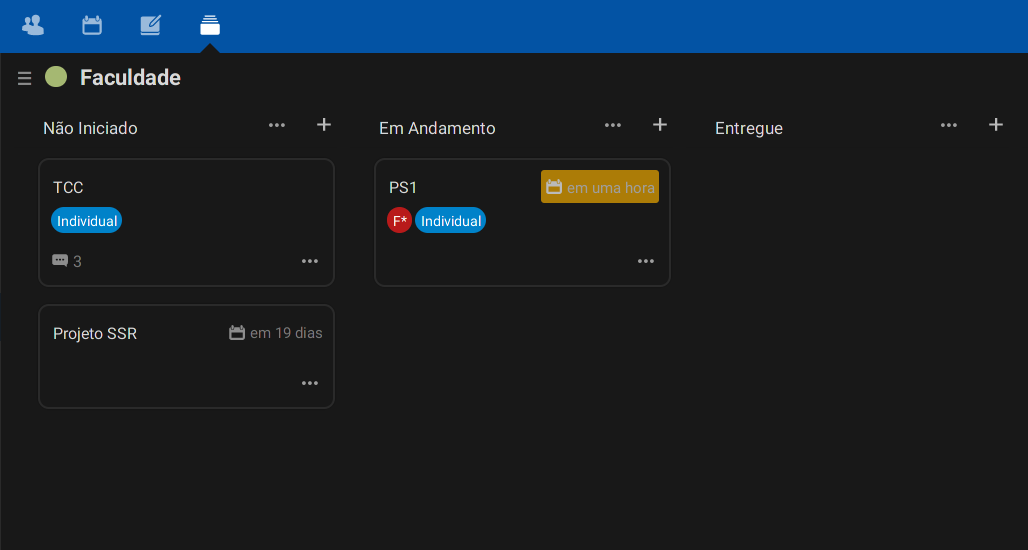
\includegraphics[width=.8\textwidth]{fig1.png}
  \caption{Tela do Aplicativo \emph{Nextcloud Deck} mostrando tarefas de um quadro}\label{fig:nexcloud-deck}
\end{figure}

\section{Desenvolvimento do Trabalho}

// Talvez falar um pouco sobre a arquitetura para justificar as linguagens

Em Maio de 2021 foi realizada pelo site~\cite{stack11}, uma pesquisa com desenvolvedores de todo o mundo para
coletar dados geográficos, sociais e de uso de tecnologias de seus usuários. Esses dados nos permitem ter
informações importantes sobre o uso de tecnologias em geral. A pesquisa nos dá três conjuntos
de informações relevantes para usarmos no trabalho

\begin{itemize}
  \item Frameworks para Web mais utilizados
  \item Frameworks gerais mais utilizados
  \item Ferramentas para deploy e gerenciamento mais usadas
  \item Banco de Dados mais utilizados
\end{itemize}

Os resultados dessas categorias, entre desenvolvedores profissionais, são exibidos nas
Figuras~\ref{fig:web-frameworks},~\ref{fig:general-frameworks},~\ref{fig:tools} e~\ref{fig:databases}, respectivamente.

\begin{figure}[H]
  \centering
  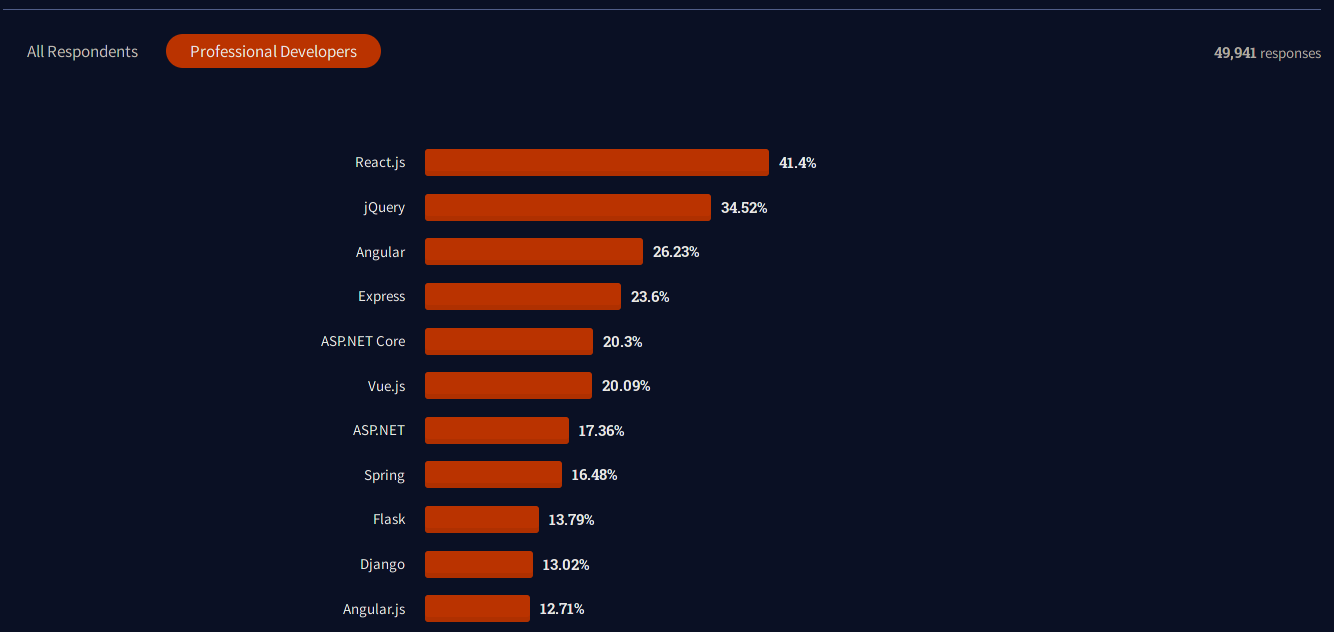
\includegraphics[width=1\textwidth]{web_frameworks_usage.png}
  \caption{Gráfico mostrando os frameworks Web mais usados}\label{fig:web-frameworks}
\end{figure}

\begin{figure}[H]
  \centering
  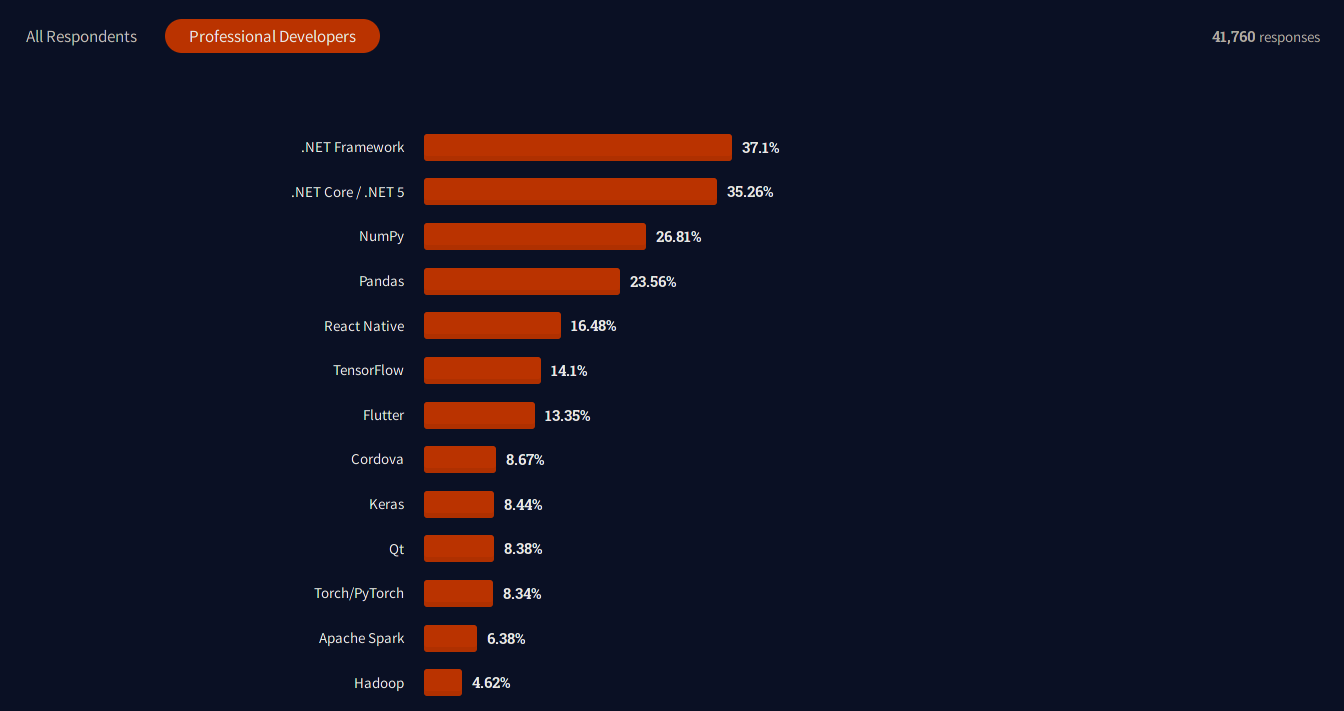
\includegraphics[width=1\textwidth]{general_framework_usage.png}
  \caption{Gráfico mostrando os frameworks gerais mais usados}\label{fig:general-frameworks}
\end{figure}

\begin{figure}[H]
  \centering
  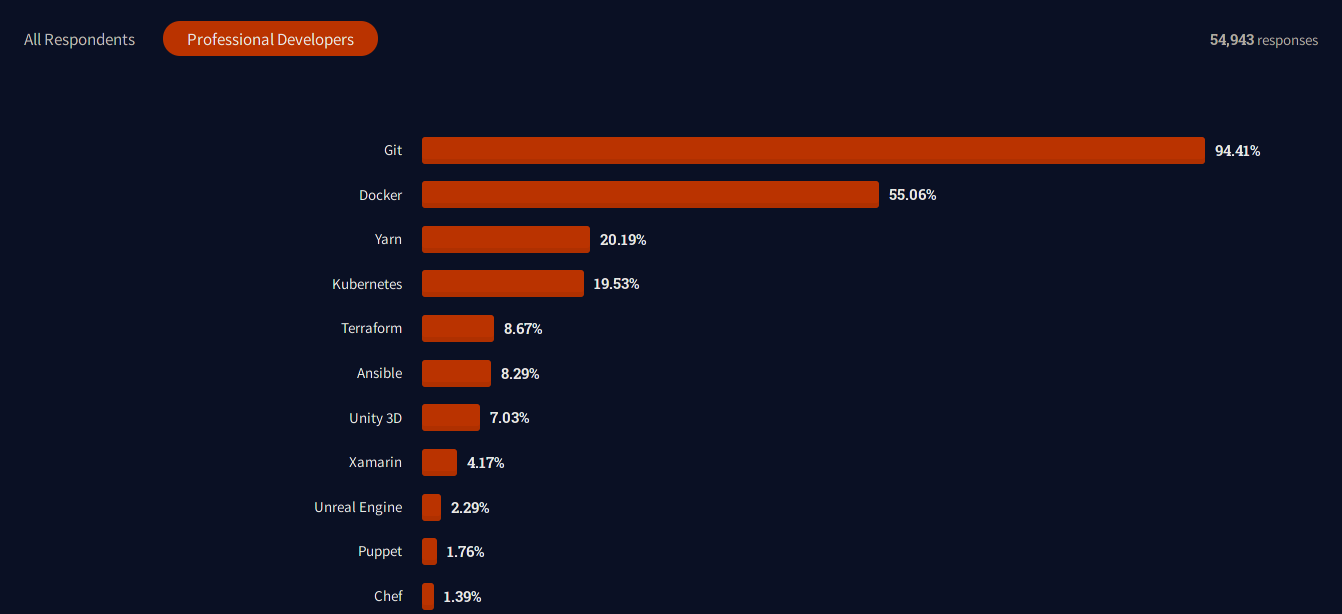
\includegraphics[width=1\textwidth]{used_tools.png}
  \caption{Gráfico mostrando as ferramentas mais usadas}\label{fig:tools}
\end{figure}

\begin{figure}[H]
  \centering
  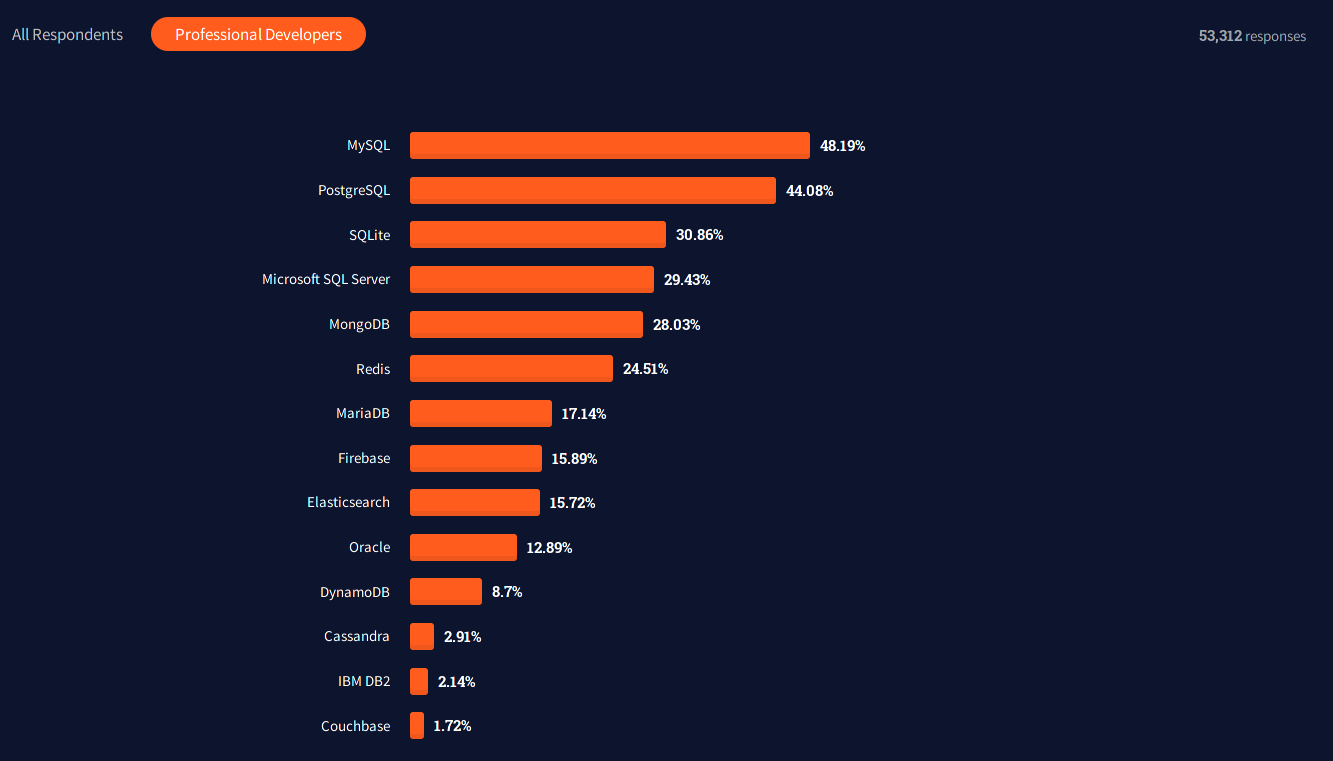
\includegraphics[width=1\textwidth]{databases.png}
  \caption{Gráfico mostrando os SGBDs mais usados}\label{fig:databases}
\end{figure}

Baseando-se nesses dados de utilização e na experiência do autor com as tecnologias, foi optado por usar as tecnologias e arquitetura
apresentadas a seguir.

\subsection{Arquitetura}

O sistema terá duas aplicações principais, uma sendo o lado do servidor (backend) e outra sendo
a aplicação que será usada pelos usuários (frontend).

O backend será desenvolvido usando o framework ASP.NET Core e
ele fornecerá um WebService RESTFul.

o frontend será uma aplicação Web que será desenvolvido com o Framework Vue.js.

\subsection{WebService}

Um WebService é um serviço que é oferecido e é por onde aplicações se comunicam com o servidor.
WebServices fazer parte da arquitetura orientada a serviços (SOA)

Um tipo de WebService muito utilizado é o REST, que significa
\emph{Representational State Transfer} ele funciona servindo requisições de clientes
para certos serviços. Por Examplo, suponha que um WebService REST tenha uma URL que fornece
informações de funcionários

\begin{verbatim}
  GET http://meuwebservice/funcionarios
\end{verbatim}

GET é o método HTTP usado para requisitar as informações que queremos, então se enviarmos uma requisição
para a URL com o método esperado, o WebService irá responder a requisição com dados em formato JSON com as informações que queremos

\begin{verbatim}
  [
    {
      "nome": "João",
      "departamento": "Contabilidade"
    },
    {
      "nome": "Bianca",
      "departamento": "Engenharia"
    }
  ]
\end{verbatim}

Um WebService REST pode ter muitas URLs, também chamadas de EndPoints.

\subsection{Spring e Java}

Java é uma linguagem hoje pertencente a Oracle e é usada em muitas aplicações.
Spring é um Framework, um conjunto de ferramentas para acelerar o desenvolvimento de aplicações.
Iremos com o Spring criar o WebService de nosso sistema e junto com uma biblioteca chamada Hibernate
iremos integrar nosso WebService com um banco de dados.

\subsection{Hibernate}

O Hibernate é um Framework para o Java que foi originalmente desenvolvido pela RedHat.
Ele é o que chamamos de ORM, um ORM é um conjunto de ferramentas que faz o mapeamento
de um banco de dados relacional para classes de Programação Orientada a Objetos.
Abaixo, um exemplo de uma classe Java mapeada para o Hibernate:

\begin{verbatim}
import javax.persistence.Entity;
import javax.persistence.GeneratedValue;
import javax.persistence.GenerationType;
import javax.persistence.Id;

import lombok.Data;

@Entity
public @Data class Person {

    @Id
    @GeneratedValue(strategy = GenerationType.IDENTITY)
    private long id;
    private String name;
    private int age;
}
\end{verbatim}

O código acima é de uma classe que representa uma Pessoa, repare nas anotações
\@Id e \@GeneratedValue, elas são chamadas Anotações e contém informações sobre algo.
Nesse caso estamos dizendo ao Hibernate que o atributo id é um atributo identificador
e que seu valor será gerado automaticamente no banco de dados. Com essas informações, o
Hibernate pode criar todos nosso banco de dados baseado nas classes e suas anotações.

\subsection{Vue.js}

O Vue é um framework para desenvolvimento de aplicações Web, usando a linguagem JavaScript,
ele nos permite o desenvolvimento de aplicações reativas e possibilita o reuso
de código através de componentes. Abaixo um pequeno código HTML de um arquivo vue

\begin{verbatim}
  <div>
    <p v-if="seen">Agora você me viu</p>
  </div>
\end{verbatim}

Esse trecho de código exibe o texto `Agora você me viu' caso a variável `seen' seja verdadeira.

O Vue nos dá a opção de usar a linguagem TypeScript ao invês do JavaScript, ele possui
várias bibliotecas que melhoram a legibilidade e arquitetura de um componente vue.
Abaixo um código de um componente Vue usando TypeScript

\begin{verbatim}
<template>
  <p>Texto</p>
</template>

<script lang="ts">
import Vue from "vue";
import Component from "vue-class-component";

@Component
export default class About extends Vue {

}
</script>
\end{verbatim}

O Vue possui um ecosistema de bibliotecas adicionais para ajudar no desenvolvimento de aplicações.

\subsection{Versionamento}

Versionamento de código é algo que sempre deve ser ultilizado, o versionamento nos ajuda a
organizar e não perder códigos escritos.

A ferramenta de versionamento que será usada é o Git e o código será hospedado na plataforma GitHub.

\section{Resultados}

O Software proposto foi completado e está dispoível junto com toda a documentação proposta no
repositório do GitHub

// Espero que esteja em breve

\section{Conclusão}

O artigo mostrou problemas existentes no ensino de desenvolvimento de software e propôs
a criação de um sistema com uma documentação abrangente para ajudar estudandes sobre alguns dos
conceitos e tecnologias usadas no desenvolvimento de software, além de prover uma abordagem prática
sobre o assunto. O Trabalho também explicou sobre conceitos de qualidade e sobre as ferramentas usadas
no desenvolvimento de software e que podem ou não serem usadas no trabalho final
que esse artigo representa.

\bibliography{bibliografia}

\end{document}
